\documentclass[lettersize,journal]{IEEEtran}

% ── Matemática ────────────────────────────────────────────────
\usepackage{amsmath,amsfonts}

% ── Algoritmos ────────────────────────────────────────────────
\usepackage{algorithmic}
\usepackage{algorithm}

% ── Tablas y arrays ───────────────────────────────────────────
\usepackage{array}
\usepackage{tabularx}
\usepackage{booktabs}

% ── Figuras y subfiguras ──────────────────────────────────────
\usepackage[caption=false,font=normalsize,labelfont=sf,textfont=sf]{subfig}
\usepackage{graphicx}
\usepackage{float}
\usepackage{stfloats}

% ── Texto y símbolos ──────────────────────────────────────────
\usepackage{textcomp}
\usepackage{url}
\usepackage{caption}
\usepackage{verbatim}
\usepackage{wasysym}

% ── Unidades SI ───────────────────────────────────────────────
\usepackage{siunitx}
\sisetup{per-mode=fraction}
\DeclareSIUnit{\inch}{in}

% ── Referencias y vínculos ────────────────────────────────────
\usepackage{cite}
\usepackage{hyperref}

% ── Cronograma Gantt ──────────────────────────────────────────
\usepackage{pgfgantt}
\usepackage{rotating}
\usepackage{xcolor}

% ── Separación de palabras ────────────────────────────────────
\hyphenation{op-tical net-works semi-conduc-tor IEEE-Xplore}

% =============================================================
\begin{document}
% =============================================================

\title{\textbf{White Paper: Diseño de un Dispositivo Trepador de Árboles}}

\author{
Cristhian Araya Chaves \texttt{criaraya@estudiantec.cr} \\
Eduardo Fallas Valverde \texttt{eduardofv@estudiantec.cr} \\
Andrés Montoya Viales \texttt{andmontoya@estudiantec.cr} \\
Jose Ignacio Morales Calvo \texttt{josmorales@estudiantec.cr} \\
Gianluca Tioli Antillon \texttt{gtioli@estudiantec.cr} \\
Aarón Valerín Páez \texttt{aavalerin@estudiantec.cr} \\
Estudiantes de Ingeniería Mecatrónica \\
Tecnológico de Costa Rica
}

\markboth{MT7006 -- Diseño de Máquinas y Mecanismos, I Semestre 2026}%
{White Paper -- Dispositivo Trepador}

\maketitle

\begin{abstract}
El presente documento corresponde a la etapa de White Paper del Proyecto Final del
curso MT7006 -- Diseño de Máquinas y Mecanismos. El objetivo general del proyecto es
el diseño conceptual de un dispositivo trepador autónomo capaz de ascender
verticalmente sobre un tronco cilíndrico de madera sin causar daño estructural al
mismo. Se establecen los requerimientos técnicos mínimos, el marco metodológico del
proceso de diseño, las restricciones del sistema y los lineamientos de evaluación
definidos por el curso.
\end{abstract}

\begin{IEEEkeywords}
Diseño mecánico, locomoción vertical, mecanismo de sujeción, trepador autónomo,
descomposición funcional.
\end{IEEEkeywords}


% ============================================================
\section{\textbf{Introducción}}
% ============================================================

El diseño de mecanismos capaces de realizar locomoción vertical sobre superficies
cilíndricas representa un desafío relevante en la ingeniería mecánica, ya que integra
aspectos de transmisión de potencia, estabilidad estructural, contacto mecánico,
fricción, adaptación geométrica y control del movimiento.

El presente proyecto consiste en concebir, diseñar y construir un prototipo mecánico
capaz de ascender de forma autónoma sobre un tronco vertical de aproximadamente
\SI{30}{\centi\meter} de diámetro y \SI{2.5}{\meter} de altura, manteniendo su
integridad estructural durante la operación y garantizando un retorno seguro a la base.
La restricción central del sistema es que no puede causar daño alguno al tronco, lo
cual elimina estrategias de penetración o adhesión y orienta el diseño hacia soluciones
de contacto distribuido y fricción controlada \cite{Vasiliauskas2001ForestryDamage,
RossnerEtAl2023BarkStripping}.

Este proyecto permite experimentar las fases completas del proceso de diseño de
ingeniería:

\begin{itemize}
    \item Generación y selección de conceptos
    \item Diseño detallado
    \item Construcción de prototipo
    \item Validación experimental
\end{itemize}

\subsection*{\textbf{Requerimientos mínimos del diseño}}

El dispositivo deberá cumplir obligatoriamente con los siguientes requerimientos:

\begin{enumerate}
    \item Altura mínima de ascenso: \SI{2}{\meter}, medida desde el punto más bajo
    del prototipo sobre el tronco.
    \item Capacidad de descenso seguro, ya sea por rutina controlada o caída libre,
    sin comprometer la integridad estructural ni funcional del dispositivo.
    \item Operación sobre tronco de madera seco, sin corteza ni ramas, de
    aproximadamente \SI{30}{\centi\meter} de diámetro y \SI{2.5}{\meter} de altura.
    \item Tolerancia a irregularidades geométricas propias del tronco real.
    \item Por sobre todo, no causar daño al tronco. Está prohibido perforar, cortar,
    ranurar, generar indentaciones o aplicar materiales adhesivos para el movimiento
    del prototipo.
\end{enumerate}

Para hacer frente al diseño a realizar, se empleará primeramente una revisión del
estado del arte para mecanismos trepadores de troncos o similares, con el fin de
identificar los distintos principios de locomoción presentes en la literatura. En base
a este estudio se realizará una descomposición funcional del sistema y se propondrá un
concepto de diseño por cada principio de locomoción identificado. Estos conceptos serán
evaluados en una matriz de decisión técnica para seleccionar los dos más prometedores,
los cuales serán desarrollados a profundidad en la etapa de diseño detallado.

% ============================================================
\section{\textbf{Estado del Arte: robots y mecanismos trepadores en troncos y postes}}
\label{sec:estado_del_arte}
% ============================================================

La locomoción vertical sobre superficies cilíndricas representa un problema mecánico
exigente. El objetivo principal del proyecto es lograr que el mecanismo pueda trepar
sobre la estructura y paralelamente conseguir que lo haga con estabilidad, continuidad
de contacto y tolerancia frente a cambios geométricos reales. Para este caso particular,
la superficie cilíndrica a utilizar será un tronco de madera de aproximadamente
\SI{30}{\centi\meter} de diámetro y \SI{2.5}{\meter} de altura, sin corteza exterior
ni ramas salientes.

Las revisiones recientes coinciden en que el desempeño de un robot trepador depende de
tres elementos principales codependientes. El primero es la manera en que el sistema
genera \textbf{fuerza normal} sobre la superficie. Seguidamente el \textbf{mecanismo}
mediante el cual esa sujeción se convierte en desplazamiento vertical. Y por último los
recursos que permiten mantener \textbf{estabilidad} y \textbf{control} cuando cambian
las condiciones de contacto \cite{FangCheng2023,DaiEtAl2023}.

Como se planteó en los requerimientos, el dispositivo no puede dañar el tronco ni usar
adhesivos. Esto descarta soluciones agresivas y obliga a diseñar mecanismos que
distribuyan el peso y ajusten la fuerza de contacto, logrando así el agarre necesario
mediante fricción sin lastimar la superficie.

La presente sección tiene como objetivo estructurar distintas soluciones y prototipos
existentes con un análisis en torno a los tres elementos principales mencionados, con
el fin de determinar qué principios de locomoción y sujeción se adaptan mejor a las
restricciones de nuestro diseño en apartados posteriores.


\subsection{\textbf{Análisis de distintos principios de locomoción en la actualidad}}

A partir de la literatura revisada, pueden distinguirse tres familias principales de
locomoción que describen de manera directa cómo se genera el
\textbf{desplazamiento vertical}. Cada una de estas familias fundamenta directamente
uno de los conceptos de diseño propuestos en la
Sección~\ref{sec:metodologia}.\\[0.3cm]

\subsubsection{\textbf{Rodadura con rodillos sincronizados}}

Una primera familia abarca los mecanismos que abrazan el tronco mediante múltiples
rodillos, transmitiendo el par a través de un sistema de sincronización o mediante
actuación independiente en cada rueda \cite{GuiTangMukhopadhyay2018}. En esta
configuración, la subida es posible gracias a que los rodillos giran coordinadamente
para transformar la fricción tangencial en desplazamiento vertical. Para mantener el
agarre, la fuerza normal es provista por un bastidor articulado de diámetro preajustable
(ver Figura~\ref{fig:bastidor_abierto}). Esto significa que la estructura se calibra a
la dimensión del tronco antes del ascenso, pero actúa como un sistema de sujeción fijo
y constante mientras el robot trepa.

\begin{figure}[htbp]
    \flushleft
    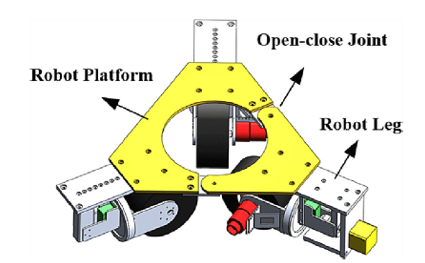
\includegraphics[width=0.5\textwidth]{Images/Ref5Image.png}
    \caption{Ejemplo de bastidor articulado para sujeción concéntrica.}
    \label{fig:bastidor_abierto}
\end{figure}

La principal ventaja de este enfoque es que permite un movimiento continuo y distribuye
de manera más homogénea la carga mecánica. Al repartir el peso y la tracción entre
varios puntos de contacto, el robot reduce la dependencia de una sola rueda para
sostenerse. Sin embargo, el reto de diseño es considerable: exige que el bastidor
mantenga una alta rigidez y alineación geométrica. Cualquier pérdida de sincronía entre
los motores o una reducción local de la fuerza normal puede traducirse rápidamente en
patinaje y pérdida de estabilidad.

Para hacer frente a estos retos, el prototipo desarrollado por Gui \emph{et al.}
\cite{GuiTangMukhopadhyay2018} propone soluciones mecánicas de gran interés que
abordan directamente el control de la sujeción y la protección de los actuadores. Su
diseño se destaca por dos aportes principales:

En primer lugar, para evitar el patinaje una de sus tres patas incorpora un motor paso a
paso (\emph{stepper}) acoplado a un mecanismo de tornillo-tuerca (husillo). Este sistema
lineal no solo ajusta el diámetro inicial del robot para troncos de entre
\SI{120}{\milli\meter} y \SI{160}{\milli\meter}, sino que actúa de forma dinámica
durante el ascenso para regular la fuerza normal entre las ruedas y la corteza.

\begin{figure}[htbp]
    \flushleft
    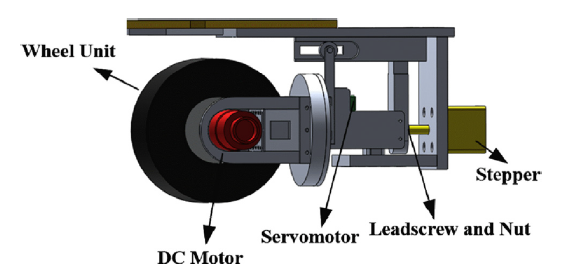
\includegraphics[width=0.55\textwidth]{Images/imagenSTepperRef5.png}
    \caption{Detalle del mecanismo de sujeción activa de Gui et al.}
    \label{fig:mecanismo_gui1}
\end{figure}

En segundo lugar, el diseño emplea servomotores para pivotar las ruedas, permitiendo
que el robot cambie su morfología de avance (pasando de un ascenso vertical a un patrón
en espiral). Para evitar fracturar los ejes de los servos por la alta fuerza normal, los
autores diseñaron un módulo de dirección compuesto por una placa rotatoria y una placa
de soporte. De esta forma, la carga estructural es absorbida por el soporte y el chasis,
aislando por completo el eje del servomotor y dando mayor estabilidad.

Finalmente, la tracción vertical queda a cargo de tres motores independientes equipados
con \emph{encoders}, lo que asegura una lectura constante de la velocidad de trepa y
permite mantener la sincronización de la rodadura en todo momento.

\begin{figure}[htbp]
    \centering
    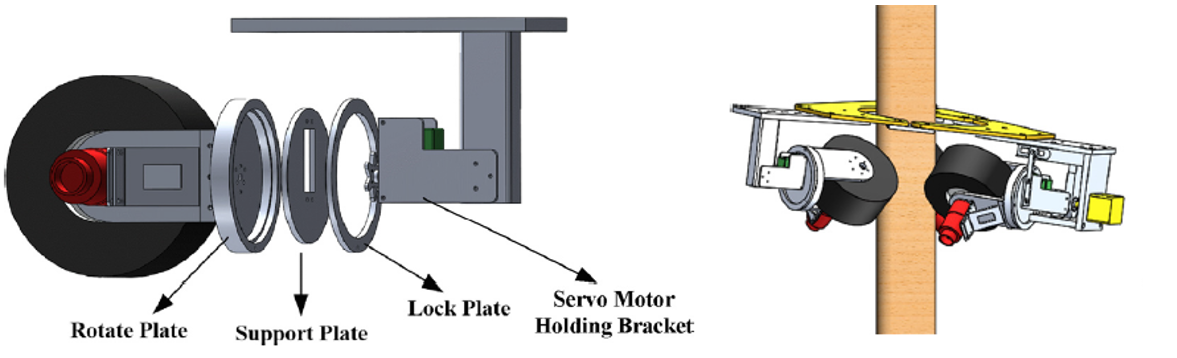
\includegraphics[width=0.55\textwidth]{Images/imagenDrivingServosRef5.png}
    \caption{Detalle del módulo de dirección de Gui et al.}
    \label{fig:mecanismo_gui2}
\end{figure}

Una alternativa mecánica distinta dentro de esta misma familia es la que presenta el
robot trepador de palmeras propuesto por Amaran \emph{et al.} \cite{Amaran2021}. En
contraste con el ajuste motorizado del diseño anterior, este prototipo soluciona el
problema de la fuerza normal y el patinaje mediante un \textbf{ajuste pasivo con
resortes de tensión} (ver Figura~\ref{fig:geometria_resorte_amaran}). Esta
configuración no solo resulta ser una opción más económica, sino que ofrece una mayor
tolerancia a cambios irregulares en la geometría del tronco. Al usar elementos
elásticos, el mecanismo absorbe las variaciones del diámetro (representadas como
$\Delta d$) y mantiene la tracción de forma automática en superficies más grandes y
rugosas.

\begin{figure}[H]
    \flushleft
    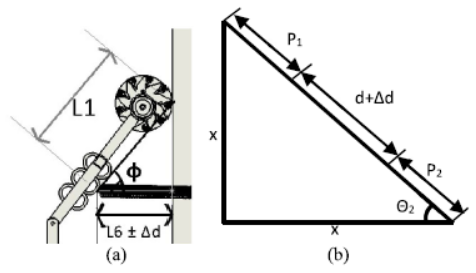
\includegraphics[width=0.5\textwidth]{Images/Ref6Spring.png}
    \caption{Vista lateral del mecanismo mostrando cómo el resorte compensa las
    variaciones en el diámetro del tronco ($\Delta d$) y su relación geométrica.}
    \label{fig:geometria_resorte_amaran}
\end{figure}

Por otro lado, para abordar el reto de las trayectorias complejas y el movimiento en
espiral, el diseño implementa \textbf{ruedas tipo Mecanum}
(ver Figura~\ref{fig:mecanum_amaran}). Estas ruedas, muy usadas actualmente en robótica
móvil, permiten la locomoción omnidireccional variando únicamente el sentido de giro de
cada rueda independiente. Esta estrategia mecánica simplifica drásticamente la
arquitectura del robot, ya que elimina la necesidad de módulos de dirección para lograr
evitar particularidades del tronco de forma sencilla.

\begin{figure}[H]
    \flushleft
    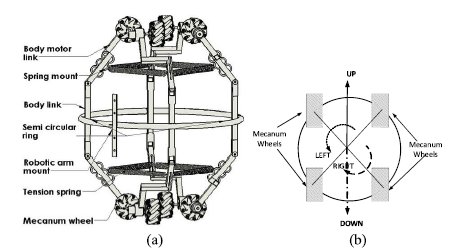
\includegraphics[width=0.5\textwidth]{Images/ManumyRobotGeneralRef6.png}
    \caption{Arquitectura del robot de Amaran et al. y diagrama de vectores para
    ruedas Mecanum.}
    \label{fig:mecanum_amaran}
\end{figure}

Por último, es válido mencionar desarrollos de mayor complejidad orientados a trabajos
pesados, como el \emph{Monkeybot} \cite{BanEtAl2022Monkeybot}. A diferencia del ajuste
por resortes en el prototipo anterior, este robot resuelve la fuerza normal mediante un
mecanismo de sujeción hidráulico (ver Figura~\ref{fig:monkeybot}). Al mantener una
presión constante en este actuador, el sistema logra adaptarse automáticamente a las
variaciones del diámetro del tronco. Asimismo, en el apartado de desplazamiento, el
diseño evoluciona al sustituir las llantas convencionales por un sistema de bandas u
orugas dobles, incrementando significativamente la superficie de contacto con la
corteza.

\begin{figure}[H]
    \flushleft
    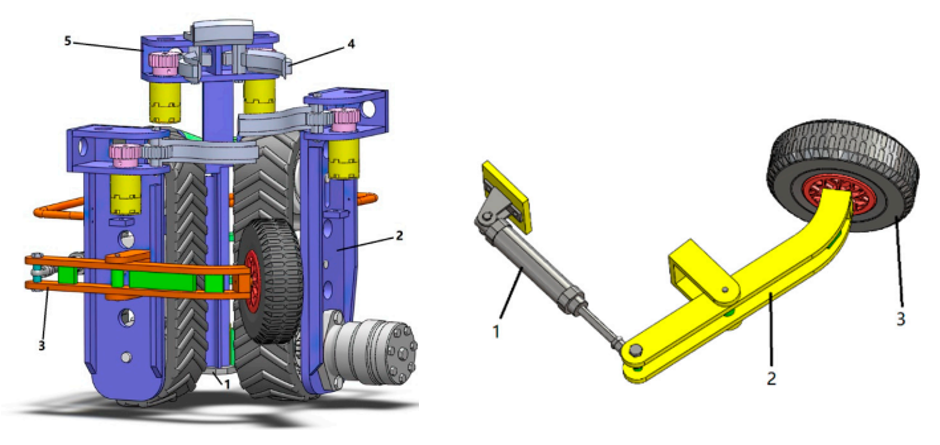
\includegraphics[width=0.50\textwidth]{Images/MonkeyBot.png}
    \caption{Monkeybot, con identificación de sus componentes principales:
    1---bastidor (frame);
    2---mecanismo de desplazamiento;
    3---mecanismo de sujeción;
    4---mecanismo de corte;
    5---mecanismo de evasión de obstáculos \cite{BanEtAl2022Monkeybot}.}
    \label{fig:monkeybot}
\end{figure}

Esta robustez ya se aproxima al diseño de cabezales procesadores utilizados en
maquinaria forestal a gran escala, como las cosechadoras de la empresa \emph{John Deere}
(ver Figura~\ref{fig:john_deere}). Sin embargo, es precisamente en este punto donde se
traza el límite para esta familia. Los equipos industriales forestales basan su agarre
en perfiles agresivos, cadenas o rodillos con púas que perforan la corteza para
maximizar la tracción. Dado que el requerimiento central del diseño a emplear exige
conservar la integridad del tronco en su totalidad, se reafirma así la necesidad de
concentrar el diseño en sistemas de \textbf{fricción no destructiva} y por ende este
modelo de sujeción se descarta.

\begin{figure}[H]
    \centering
    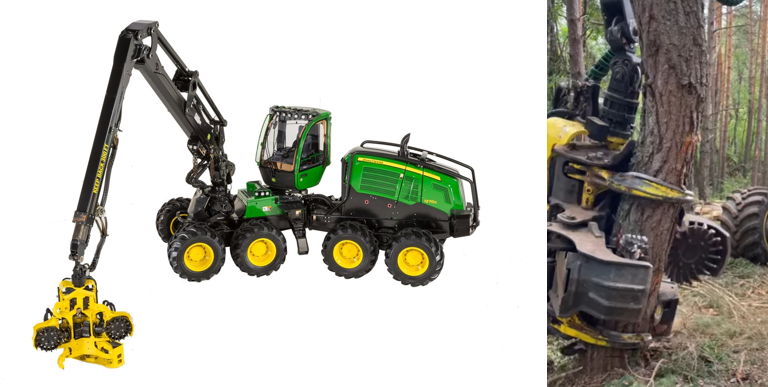
\includegraphics[width=0.5\textwidth]{Images/JohnDeereImage.png}
    \caption{Cabezal procesador de una cosechadora forestal, marca John Deere.}
    \label{fig:john_deere}
\end{figure}

\newpage

\subsubsection{\textbf{Locomoción alternante por módulos de agarre y cuerpo extensible}}

En esta familia el ascenso no se produce por rodadura continua, sino por una secuencia
repetida en la que un módulo de agarre sostiene el sistema mientras otro avanza y se
fija en una posición superior. Luego el primer módulo se libera, el cuerpo cambia de
longitud o de postura, y el ciclo vuelve a empezar. El desplazamiento vertical nace
entonces de una \textbf{alternancia} entre sujeción y rearme mecánico.

\begin{figure}[H]
    \centering
    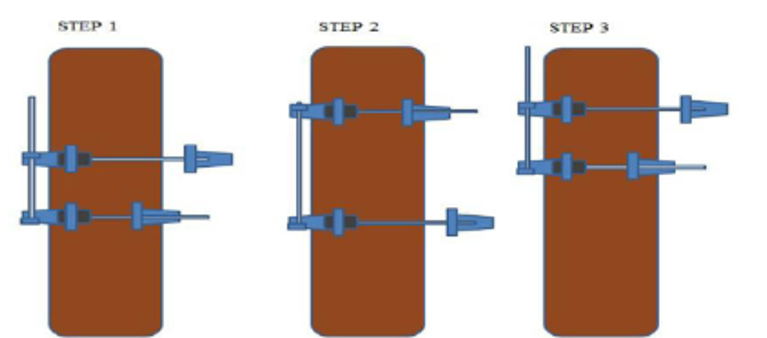
\includegraphics[width=0.5\textwidth]{Images/AlternanciaImage.png}
    \caption{Mecanismo alternante ejemplo gráfico \cite{WangDuZhangXue2021WLPCR}.}
    \label{fig:alernancia}
\end{figure}

Por lo mencionado anteriormente, durante buena parte del ciclo existe al menos un punto
de apoyo firme, lo que reduce el riesgo de caída ante una pérdida puntual de tracción.
Esa ventaja suele venir acompañada de una estructura más articulada y de tiempos de
avance menores.

El robot Treebot muestra cómo un cuerpo extensible y una estrategia de trepa táctil
pueden adaptarse a superficies irregulares \cite{LamXu2011ICRA}.

\begin{figure}[H]
    \flushleft
    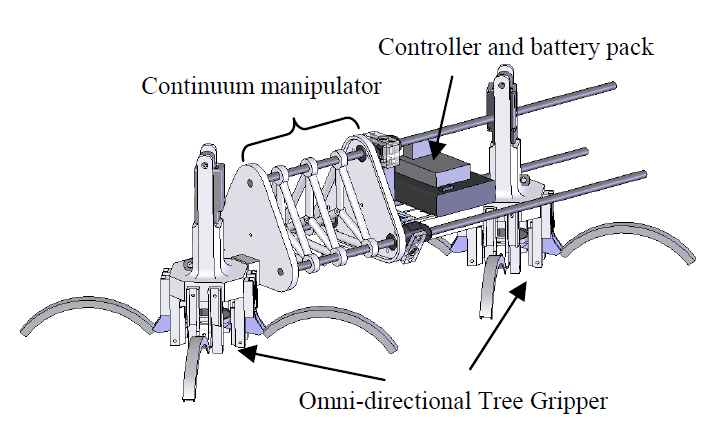
\includegraphics[width=0.47\textwidth]{Images/TreeBot15_8Image.png}
    \caption{Robot Treebot \cite{LamXu2011ICRA}.}
    \label{fig:treebotgeneral}
\end{figure}

Un aspecto destacado de este prototipo es el diseño de sus \textbf{módulos de agarre
omnidireccionales} (ver Figura~\ref{fig:gripper_treebot}). Esta morfología le otorga al
robot una alta maniobrabilidad, ya que inclusive ramas salientes no serían un
inconveniente. Como se observa en su esquema cinemático, al retraer el motor lineal, una
placa de empuje obliga a las uniones a cerrarse contra el tronco, emulando la
biomecánica de un animal escalador. Por su parte, un conjunto de resortes mecánicos
actúa como sistema de retorno pasivo para abrir las garras una vez que el motor avanza.

\begin{figure}[H]
    \centering
    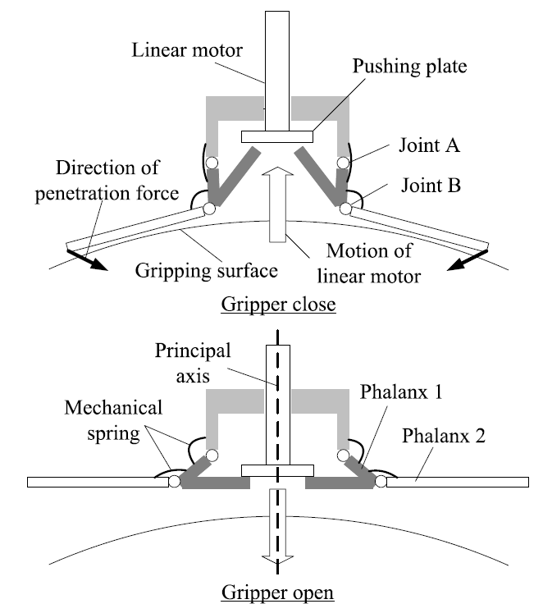
\includegraphics[width=0.4\textwidth]{Images/gripperTreebot.png}
    \caption{Cinemática del módulo de agarre del Treebot: estados de apertura y cierre
    accionados por un motor lineal.}
    \label{fig:gripper_treebot}
\end{figure}

Si bien la cinemática de extensión y contracción del cuerpo resulta ideal para adaptarse
a superficies complejas, es importante notar que su principio de sujeción depende
intrínsecamente de fuerzas de penetración. Por lo tanto, su agarre resulta incompatible
con la restricción de este proyecto de conservar la integridad del tronco.

Como aspecto innovador para lograr el desplazamiento entre ambos puntos de agarre, el
\emph{Treebot} sustituye los chasis rígidos por un cuerpo extensible basado en un
manipulador continuo (\emph{continuum manipulator}). A diferencia de los actuadores
lineales convencionales, este sistema utiliza tres resortes mecánicos paralelos que
operan como ``cremalleras flexibles'', impulsadas independientemente por un sistema de
piñón y motor.

\begin{figure}[H]
    \centering
    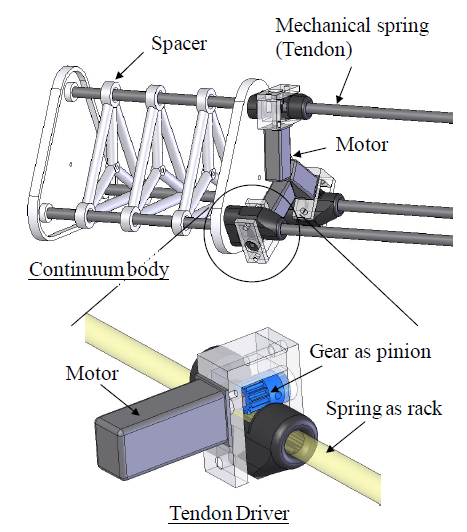
\includegraphics[width=0.38\textwidth]{Images/ContiniumManipulator.png}
    \caption{Vista de detalle del \emph{continuum manipulator}.}
    \label{fig:continumManipulator}
\end{figure}

Al variar la longitud relativa de cada resorte, el cuerpo del robot genera un
diferencial de extensión que le permite no solo elongarse, sino \textbf{flexionarse
omnidireccionalmente} (alcanzando 3 grados de libertad,
ver Figura~\ref{fig:Degreesoffreedom}). Esta flexibilidad estructural le otorga la
capacidad de arquearse para sortear irregularidades y adaptar su postura a la curvatura
natural del árbol.

\begin{figure}[H]
    \centering
    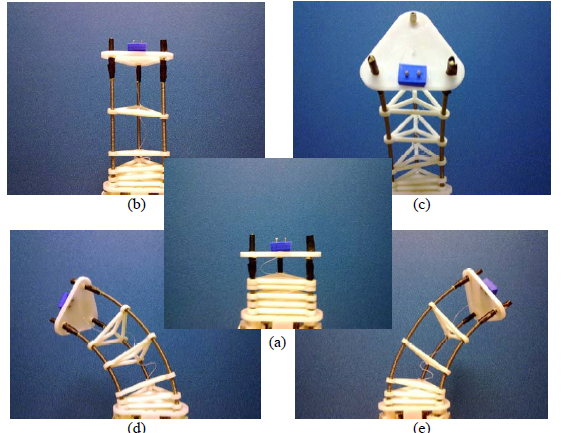
\includegraphics[width=0.4\textwidth]{Images/DegreesOfFreedoomdelMAnipulador.png}
    \caption{Distintos ángulos de libertad del robot, prototipo real TreeBot.}
    \label{fig:Degreesoffreedom}
\end{figure}

Dentro de esta misma lógica de locomoción alternante, existe una variante constructiva
que sustituye la extensión del cuerpo por un \textbf{avance lineal rígido mediante
husillo} (mecanismo tornillo-tuerca) \cite{DubeyEtAl2016Coconut}. En este enfoque, un
módulo de agarre se fija al tronco mientras el tornillo motorizado empuja el resto de la
estructura hacia arriba.

\begin{figure}[H]
    \centering
    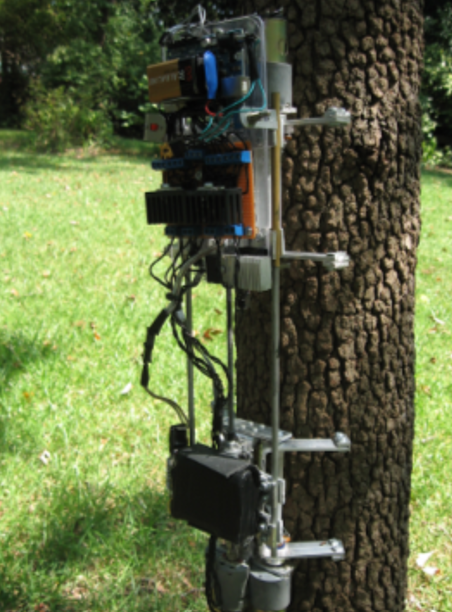
\includegraphics[width=0.35\textwidth]{Images/TornilloSinFinDiseño.png}
    \caption{Prototipo de locomoción alternante por avance de husillo propuesto
    por Katz.}
    \label{fig:husillo_katz}
\end{figure}

Esta alternativa, explorada en configuraciones compactas como las de Katz
\cite{Katz2011TreeClimbing}, resulta muy atractiva por una razón fundamental de
seguridad: la \textbf{retención pasiva}. El mecanismo roscado es inherentemente
autobloqueante, lo que significa que el robot no caerá ante una pérdida súbita de
potencia. Dado que el desplazamiento máximo por ciclo está dictado por la longitud del
tornillo, escalar este diseño para trepar alturas del orden de \SI{2}{\meter} obligaría
a integrar un husillo de grandes dimensiones, y movilizar el mecanismo sería
particularmente lento.\\[0.3cm]

\subsubsection{\textbf{Locomoción por palanca}}

Esta última familia de mecanismos se basa en un principio biomecánico, directamente en
la técnica que utilizan los seres humanos para escalar árboles o postes mediante arneses
(ver Figura~\ref{fig:inspiracion_humana}). En este enfoque, la fuerza normal necesaria
para evitar el deslizamiento no proviene de actuadores que contraigan la estructura
contra el tronco, sino principalmente del mismo peso por gravedad de la estructura.

\begin{figure}[H]
    \centering
    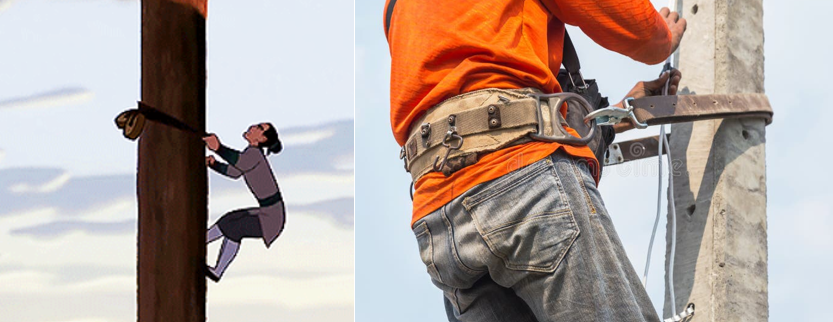
\includegraphics[width=0.45\textwidth]{Images/LocomocionHumanInspired.png}
    \caption{Principio biomecánico: el peso del escalador genera la fuerza de sujeción
    a través de un brazo de palanca.}
    \label{fig:inspiracion_humana}
\end{figure}

Constructivamente, el robot se diseña proyectando su centro de masa lejos del eje
longitudinal del tronco. Al suspenderse, la estructura principal actúa como un brazo de
palanca que obliga a los puntos de contacto (superior e inferior) a presionarse
fuertemente contra la corteza (ver Figura~\ref{fig:robot_palanca}).

\begin{figure}[H]
    \centering
    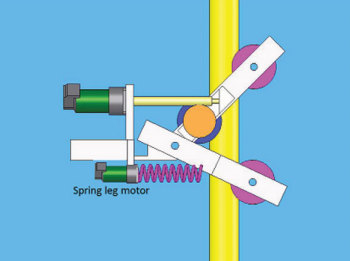
\includegraphics[width=0.40\textwidth]{Images/RobotConPalancaChristian.png}
    \caption{Esquema estructural de un robot trepador por palanca, destacando los
    puntos de apoyo y el actuador de inclinación
    \cite{Sadeghi2012HumanInspired}.}
    \label{fig:robot_palanca}
\end{figure}

Esta estrategia de \textbf{bloqueo gravitacional} resulta extremadamente eficiente desde
el punto de vista energético, ya que el sistema no requiere consumir potencia eléctrica
para mantenerse firmemente aferrado al árbol en estado de reposo.

Por ejemplo, la versión de cortador de fruta de esta familia es el robot desarrollado
por Zhen \emph{et al.} \cite{ZHENG2024100617}. Omitiendo la herramienta superior de
recolección, el diseño mecánico de su sistema de locomoción aporta una solución para el
control del bloqueo gravitacional.

Para gestionar el ascenso y la adaptación al tronco, el prototipo además de una palanca
estática implementa un \textbf{ajuste activo del ángulo de sujeción} utilizando un
actuador lineal combinado con un resorte de gas
(ver Figura~\ref{fig:estructura_zhen}). El actuador lineal permite modificar la apertura
entre el chasis principal (\emph{frame}) y el brazo de sujeción (\emph{clamping arm}).
Al retraerse, disminuye la fuerza normal para facilitar la rodadura hacia arriba; al
extenderse, asegura el bloqueo. Por su parte, el resorte de gas actúa como un elemento
de cumplimiento pasivo (\emph{passive compliance}), absorbiendo impactos y manteniendo
una presión constante a pesar de las irregularidades de la corteza.

\begin{figure}[H]
    \centering
    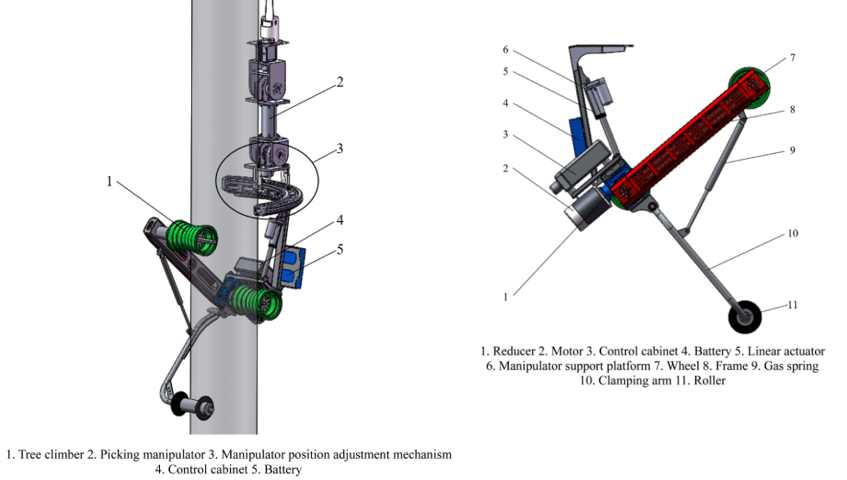
\includegraphics[width=0.5\textwidth]{Images/ZhenEtAllPoleActuadorLineal.png}
    \caption{Estructura esquemática del robot trepador de Zhen et al., destacando el
    actuador lineal (5) y el resorte de gas (9) para el control del brazo de
    sujeción.}
    \label{fig:estructura_zhen}
\end{figure}

Otro aporte de este diseño es su sistema de transmisión. Para optimizar el efecto de
palanca, el motor de tracción y la reductora se ubican en la parte inferior del chasis,
alejando el centro de masa del tronco. Sin embargo, para añadir tracción también emplean
una transferencia de potencia a la llanta superior sin añadir peso extra en la punta.
Para realizar esto, el diseño incorpora un \textbf{eje de transmisión rígido
sincronizado mediante engranajes cónicos} (\emph{bevel gears}), como se detalla en la
Figura~\ref{fig:transmision_zhen}. Esta configuración asegura que ambas ruedas giren a
la misma velocidad, maximizando el aprovechamiento de la fuerza de fricción y
previniendo el patinaje.

\begin{figure}[H]
    \centering
    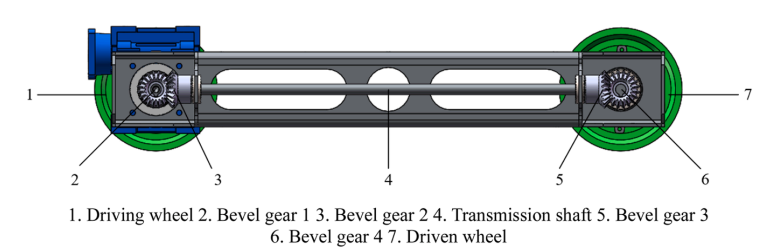
\includegraphics[width=0.5\textwidth]{Images/ZhenEtAllPoleTrasmisionn.png}
    \caption{Mecanismo de transmisión de potencia de Zhen et al., utilizando un eje
    central y engranajes cónicos para sincronizar la rodadura.}
    \label{fig:transmision_zhen}
\end{figure}

Como una alternativa mecánica más simple frente al uso de resortes de gas o actuadores
lineales, destacan los diseños propuestos por Sibasad \emph{et al.} \cite{sibasad2017}
y Sadeghi \emph{et al.} \cite{Sadeghi2012HumanInspired}. Estas arquitecturas optan por
utilizar \textbf{resortes de tensión convencionales} para aumentar pasivamente la
tracción y asegurar la fuerza normal del sistema contra el tronco
(ver Figura~\ref{fig:resorte_sadeghi}).

Cabe destacar que estos diseños no utilizan sistemas de transmisión complejos para
sincronizar múltiples ruedas. Estos concentran la masa del motor en un solo extremo para
desplazar intencionalmente el centro de gravedad y la potencia se transfiere de forma
directa y exclusiva al rodillo más cercano a esta masa (rueda motriz), dejando el resto
de los rodillos como apoyos pasivos de giro libre. Esta alternativa resulta de gran
utilidad para el diseño conceptual, ya que al evitar una cantidad excesiva de actuadores
y ejes de transmisión, se reduce drásticamente el peso general y se simplifica la
electrónica de control.

\begin{figure}[H]
    \centering
    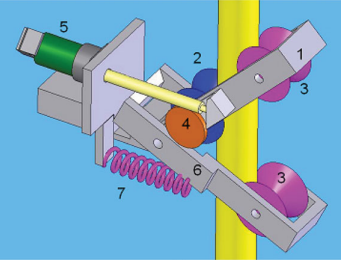
\includegraphics[width=0.35\textwidth]{Images/RobotConPalancaChristian2.png}
    \caption{Diseño bioinspirado con resorte de tensión (7) y tracción concentrada en
    una única rueda motriz (4) \cite{Sadeghi2012HumanInspired}.}
    \label{fig:resorte_sadeghi}
\end{figure}


\subsection{\textbf{Modelado mínimo del agarre: fricción y presión de contacto}}

Parte de la literatura además destaca que un modelo de primer orden permite fijar
condiciones mínimas de diseño sin recurrir aún a simulaciones complejas. Para un robot
de masa $m$ en ascenso a velocidad constante, la condición de no deslizamiento se logra
definir según la ecuación~\ref{eq:friccion}.

\begin{equation}
\mu N_{\text{tot}} \geq S_f m g,
\label{eq:friccion}
\end{equation}

Donde $\mu$ es el coeficiente de fricción efectivo entre el material de contacto y la
madera, $N_{\text{tot}}$ es la fuerza normal total aplicada al tronco y $S_f$ es un
factor de seguridad. Esta expresión es útil como punto de partida, pero no debe
interpretarse como si la fricción fuera un valor estático. La literatura sobre
elastómeros demuestra que $\mu$ varía significativamente con la rugosidad, la velocidad
de deslizamiento, el estado de precontacto y las condiciones térmicas
\cite{KaiserEtAl2024ElastomerFriction,PerssonXu2025RubberFriction}.

Esto implica que un concepto mecánico puede parecer suficiente en el papel, pero fallar
en la práctica si fue concebido con un valor de fricción demasiado optimista. Por esta
razón, los trabajos consultados coinciden en la necesidad de ampliar el área de
contacto, regular de forma consistente la fuerza normal y complementar el mecanismo
principal con recursos de seguridad (como resortes o bloqueos pasivos) que mantengan
el sistema contenido ante eventuales pérdidas de tracción
\cite{GuiTangMukhopadhyay2018,FaurouxMorillon2010SelfLock}.

Por otro lado, la integridad estructural del propio mecanismo de sujeción depende de
manera directa de la presión de contacto generada, la cual puede aproximarse según la
fórmula~\ref{eq:presion}.

\begin{equation}
p \approx \frac{N_{\text{tot}}}{A_{\text{cont}}},
\label{eq:presion}
\end{equation}

Donde $A_{\text{cont}}$ es el área efectiva de contacto. Aumentar esta área no solo
estabiliza el agarre, sino que reduce drásticamente la presión puntual. En el ámbito de
los robots trepadores, esta relación constituye un criterio limitante crítico. Como
señalan Sadeghi \emph{et al.} \cite{Sadeghi2012HumanInspired}, la carga máxima
admisible del sistema está restringida por la resistencia mecánica de los elementos de
contacto para evitar su deformación prematura.

Desde la perspectiva del análisis estático, modelar esta presión permite garantizar que
los esfuerzos de compresión concentrados no superen el límite de fluencia de los
recubrimientos o llantas del robot \cite{Shigley2020}. Dimensionar el área de contacto
para mantener estos esfuerzos dentro del rango elástico previene deformaciones plásticas
permanentes y fallos por fatiga superficial, estableciendo así un parámetro cuantitativo
y seguro para el dimensionamiento de los componentes inicialmente.

Para finalizar, la revisión del estado del arte evidencia que la locomoción vertical no
destructiva exige un equilibrio entre la fuerza de sujeción generada y la arquitectura
del mecanismo. El análisis comparativo de las tres familias identificadas ---
\textbf{rodadura sincronizada}, \textbf{avance alternante} y \textbf{locomoción por
palanca} --- permitirá fundamentar una matriz de decisión objetiva en apartados
posteriores, garantizando que cada concepto propuesto corresponde a un principio de
locomoción distinto y documentado en la literatura.

% ============================================================
\section{\textbf{Objetivos}}
% ============================================================

\subsection{\textbf{Objetivo General}}

Diseñar y construir un prototipo funcional de dispositivo trepador autónomo capaz de
ascender al menos \SI{2}{\meter} sobre un tronco cilíndrico de madera, cumpliendo los
requerimientos técnicos establecidos mediante la aplicación de una metodología
estructurada de diseño de productos mecánicos.

\subsection{\textbf{Objetivos Específicos}}

\begin{enumerate}

    \item \textbf{Identificar} los principios de locomoción vertical documentados en
    la literatura técnica y los criterios de diseño relevantes para el contexto de
    esta consigna, mediante una revisión bibliográfica sistemática de al menos 15
    fuentes.

    \item \textbf{Aplicar} una metodología estructurada de descomposición funcional al
    sistema trepador, definiendo subsistemas, entradas y salidas, para generar un
    concepto de diseño por cada principio de locomoción identificado en el estado del
    arte.

    \item \textbf{Evaluar} los conceptos propuestos mediante una matriz de decisión
    técnica ponderada con criterios objetivos trazables a la literatura, seleccionando
    los dos conceptos con mayor puntaje para su desarrollo en la etapa de diseño
    detallado.

    \item \textbf{Desarrollar} el diseño detallado de los dos conceptos seleccionados,
    incluyendo memoria de cálculos, simulaciones mecánicas y planos técnicos que
    verifiquen el cumplimiento de los requerimientos estructurales y funcionales,
    seleccionando el prototipo final con base en los resultados obtenidos.

    \item \textbf{Construir} y validar experimentalmente el prototipo final
    seleccionado, demostrando su capacidad de ascender al menos \SI{2}{\meter} y
    retornar a la base de forma segura sin causar daño al tronco, en un mínimo de
    tres ciclos completos.

    \item \textbf{Documentar} de forma continua y rigurosa todo el proceso de diseño
    en la bitácora digital del equipo, registrando decisiones técnicas, reuniones,
    evidencias multimedia y avances semanales de cada integrante.

\end{enumerate}


% ============================================================
\section{\textbf{Metodología}}
\label{sec:metodologia}
% ============================================================

La metodología sigue un enfoque estructurado de diseño de productos basado en
descomposición funcional, generación sistemática de conceptos y selección mediante
matriz de decisión técnica ponderada, siguiendo los lineamientos de Ulrich y
Eppinger \cite{UlrichEppinger2012}.

% ------------------------------------------------------------
\subsection{\textbf{Descomposición funcional}}
% ------------------------------------------------------------

El sistema se concibe como una caja negra que recibe energía eléctrica almacenada
y produce desplazamiento vertical ascendente sobre el tronco. La descomposición en
subfunciones se presenta en la Tabla~\ref{tab:descomposicion}.

\begin{table}[H]
\centering
\caption{Descomposición funcional del sistema trepador.}
\label{tab:descomposicion}
\footnotesize
\begin{tabular}{p{0.28\linewidth} p{0.30\linewidth} p{0.30\linewidth}}
\toprule
\textbf{Subfunción} & \textbf{Entrada} & \textbf{Salida} \\
\midrule
Almacenar energía
    & Energía eléctrica (carga)
    & Energía disponible para actuadores \\
Generar fuerza normal
    & Energía mecánica / resortes
    & Fuerza de sujeción radial sobre el tronco \\
Convertir energía en torque
    & Energía eléctrica
    & Par mecánico en eje de tracción \\
Transmitir movimiento
    & Par mecánico
    & Velocidad y fuerza en punto de contacto \\
Producir desplazamiento vertical
    & Fuerza de tracción + sujeción
    & Ascenso o descenso sobre el tronco \\
Mantener estabilidad lateral
    & Fuerzas externas / geometría del tronco
    & Equilibrio sin rotación alrededor del eje \\
Gestionar retorno
    & Señal de control / gravedad
    & Descenso seguro a la base del tronco \\
Controlar el sistema
    & Señales de sensores / comandos
    & Señales de activación para los actuadores \\
\bottomrule
\end{tabular}
\end{table}

% ------------------------------------------------------------
\subsection{\textbf{Conceptos de diseño propuestos}}
% ------------------------------------------------------------

Con base en la descomposición funcional y en las tres familias de locomoción
identificadas en el estado del arte, se propone un concepto de diseño por cada
familia. Esta correspondencia directa garantiza que los conceptos evaluados son
fundamentalmente distintos entre sí y están respaldados por la literatura revisada.

\subsubsection{Concepto 1 -- Escalador por rodillos sincronizados con resortes de
tensión}

Este concepto pertenece a la familia de \textbf{rodadura con rodillos sincronizados}.
Utiliza un bastidor que abraza el tronco con múltiples ruedas motrices dispuestas
radialmente, accionadas por motores independientes con \emph{encoders} para mantener
la sincronización. La fuerza normal se genera y mantiene pasivamente mediante
\textbf{resortes de tensión}, los cuales absorben además las variaciones locales de
diámetro del tronco sin intervención del sistema de control
\cite{Amaran2021, GuiTangMukhopadhyay2018}. La tracción vertical es distribuida entre
todos los puntos de contacto simultáneamente, lo que reduce el riesgo de patinaje
por concentración de carga. Las ruedas en contacto directo con la superficie del tronco
generan simultáneamente la fuerza normal y la tracción vertical
(ver Figura~\ref{fig:geometria_resorte_amaran}).

\textbf{Ventajas:} movimiento continuo sin ciclos alternantes, distribución homogénea
de la carga mecánica entre múltiples puntos de contacto, adaptación pasiva a
irregularidades del tronco mediante los resortes y componentes de alta disponibilidad
comercial.

\textbf{Limitaciones:} requiere sincronización entre múltiples motores, el bastidor
debe mantener rigidez geométrica suficiente para que la precarga de los resortes sea
efectiva, y la pérdida de sincronía puede traducirse en patinaje
\cite{GuiTangMukhopadhyay2018}.

\textbf{Trazabilidad funcional:} este concepto aborda principalmente las subfunciones
\emph{Generar fuerza normal} (resortes de tensión), \emph{Transmitir movimiento}
(motores sincronizados) y \emph{Producir desplazamiento vertical}
(Tabla~\ref{tab:descomposicion}). La subfunción \emph{Gestionar retorno} se resuelve
por inversión coordinada de los motores. La subfunción \emph{Controlar el sistema}
es la de mayor complejidad en este concepto, al requerir lazo de control para
sincronización.

\subsubsection{Concepto 2 -- Escalador alternante por módulos de agarre}

Este concepto pertenece a la familia de \textbf{locomoción alternante}. Emplea dos
módulos de agarre independientes que abrazan el tronco en puntos distintos: mientras
uno sostiene el sistema firmemente, el otro libera su sujeción, avanza hacia arriba y
vuelve a fijarse. Luego invierten roles y el ciclo se repite. El desplazamiento
vertical emerge de esta alternancia entre sujeción y rearme mecánico
\cite{LamXu2011ICRA, Katz2011TreeClimbing}. La fuerza normal en cada módulo se genera
por el cierre mecánico de los brazos de agarre, cuyo principio de operación se
inspira en la biomecánica de primates escaladores
(ver Figura~\ref{fig:gripper_treebot}).

\textbf{Ventajas:} durante la mayor parte del ciclo existe al menos un punto de
agarre firme, lo que confiere seguridad intrínseca ante pérdidas puntuales de
tracción; el retorno puede realizarse invirtiendo la secuencia de alternancia.

\textbf{Limitaciones:} mayor complejidad mecánica y de control para coordinar los
dos módulos alternantes; propenso a fallas por holguras acumuladas en las
articulaciones bajo carga repetida; velocidad de ascenso inferior a los conceptos
de rodadura continua \cite{DubeyEtAl2016Coconut}.

\textbf{Trazabilidad funcional:} este concepto aborda las subfunciones \emph{Generar
fuerza normal} (cierre mecánico de los módulos), \emph{Producir desplazamiento
vertical} (alternancia de módulos) y \emph{Mantener estabilidad lateral} (punto de
agarre firme permanente) de la Tabla~\ref{tab:descomposicion}. La subfunción
\emph{Gestionar retorno} se resuelve por la secuencia inversa de alternancia, siendo
el concepto más robusto en este criterio ya que siempre existe un punto de anclaje.

\subsubsection{Concepto 3 -- Escalador por palanca con resortes de tensión}

Este concepto pertenece a la familia de \textbf{locomoción por palanca}. Se inspira
directamente en la biomecánica del escalado humano con arnés, donde el peso del
escalador genera la fuerza de sujeción a través de un brazo de palanca
\cite{Sadeghi2012HumanInspired, sibasad2017}. El chasis se diseña de forma
asimétrica, proyectando deliberadamente el centro de masa lejos del eje longitudinal
del tronco. Al suspenderse sobre este, la estructura actúa como un brazo de palanca
que obliga a los puntos de contacto superior e inferior a presionarse contra la
superficie sin necesidad de actuadores de sujeción activos
(ver Figura~\ref{fig:robot_palanca}).

La fuerza normal se genera y mantiene pasivamente mediante \textbf{resortes de
tensión convencionales}, los cuales además absorben las variaciones locales de
diámetro del tronco sin intervención del sistema de control
\cite{Sadeghi2012HumanInspired}. La tracción vertical se concentra en una
\textbf{única rueda motriz} ubicada en el extremo inferior del chasis, donde
también se localiza la masa del motor para maximizar el efecto de palanca. El
resto de los rodillos actúan como apoyos pasivos de giro libre, lo que simplifica
drásticamente la electrónica de control al requerir un solo driver de motor. El
descenso puede realizarse invirtiendo el sentido de giro del motor o mediante
caída libre controlada, dado que la sujeción pasiva mantiene la integridad
estructural del dispositivo durante todo el proceso
\cite{sibasad2017, ZHENG2024100617}.

\textbf{Ventajas:} bloqueo gravitacional pasivo sin consumo energético en reposo,
arquitectura de pocas piezas con alta disponibilidad comercial, control de un único
actuador, adaptación pasiva a irregularidades del tronco mediante los resortes, y
descenso seguro sin lógica de control adicional.

\textbf{Limitaciones:} el efecto de palanca genera un momento de vuelco que debe ser
contenido por el diseño geométrico del chasis; la fuerza normal depende del peso
total del sistema, por lo que componentes muy livianos pueden resultar insuficientes
para mantener la tracción; requiere una calibración inicial de la tensión de los
resortes para el diámetro específico del tronco de \SI{30}{\centi\meter}.

\textbf{Trazabilidad funcional:} este concepto es el de mayor eficiencia en la
subfunción \emph{Generar fuerza normal}, ya que la resuelve pasivamente mediante el
efecto de palanca gravitacional sin consumo energético \cite{Sadeghi2012HumanInspired}.
Las subfunciones \emph{Convertir energía en torque} y \emph{Producir desplazamiento
vertical} se concentran en un único actuador, simplificando al mínimo la subfunción
\emph{Controlar el sistema} (Tabla~\ref{tab:descomposicion}). La subfunción
\emph{Gestionar retorno} se resuelve pasivamente por la misma sujeción gravitacional
durante la caída libre controlada.

% ------------------------------------------------------------
\subsection{\textbf{Lectura comparativa de los conceptos propuestos}}
% ------------------------------------------------------------

Antes de asignar puntajes en la matriz de decisión, conviene dejar claro qué aspectos
pueden debilitar a cada propuesta. En el criterio de \emph{cumplimiento de no daño},
pierden valor los conceptos que concentran la carga en áreas pequeñas o que podrían
requerir deslizamiento repetido sobre la superficie para mantener el avance
\cite{Vasiliauskas2001ForestryDamage}. En \emph{retorno seguro}, se penalizan las
soluciones que dependen por completo del control activo o del suministro continuo de
energía para no perder estabilidad durante el descenso
\cite{FaurouxMorillon2010SelfLock}.

En \emph{adaptación al diámetro e irregularidades}, tienden a puntuar más bajo los
mecanismos demasiado rígidos o con ventanas estrechas de ajuste \cite{Amaran2021}. En
\emph{margen anti-deslizamiento}, bajan de puntaje las propuestas que trabajan
demasiado cerca del límite de fricción o que dependen de un coeficiente de fricción
optimista \cite{KaiserEtAl2024ElastomerFriction}. En \emph{complejidad y
fabricabilidad}, se castigan los conceptos que requieren muchas piezas especiales o
tolerancias difíciles de sostener en un prototipo estudiantil
\cite{UlrichEppinger2012}.

Un concepto pierde puntos en \emph{estabilidad global} cuando el centro de masa queda
muy alejado del tronco o cuando la geometría hace difícil contener momentos de vuelco
\cite{Sadeghi2012HumanInspired}. En \emph{complejidad de control}, se penalizan las
propuestas que exigen sincronización muy fina entre varios actuadores
\cite{GuiTangMukhopadhyay2018}. Finalmente, en \emph{viabilidad de construcción}, se
penalizan los conceptos cuya fabricación requiere procesos especializados o tiempos de
manufactura incompatibles con el plazo del proyecto \cite{DubeyEtAl2016Coconut}.

% ------------------------------------------------------------
\subsection{\textbf{Matriz de decisión técnica}}
% ------------------------------------------------------------

Los tres conceptos se evalúan con base en ocho criterios derivados del estado del arte,
cada uno con un peso relativo asignado según su relevancia para el cumplimiento de los
requerimientos mínimos. La escala de puntuación es de 1 a 5, donde 1 indica la
puntuación mínima y 5 el máximo de puntos posibles respecto al criterio evaluado. El
puntaje ponderado de cada celda se obtiene como $\text{WP} = P \times w$.

\begin{table*}[ht]
\centering
\caption{Matriz de decisión técnica ponderada (3 conceptos). P:~puntuación (1--5);
         WP:~puntaje ponderado ($P \times w$). Conceptos seleccionados subrayados.}
\label{tab:matriz_decision}
\footnotesize
\setlength{\tabcolsep}{4pt}
\begin{tabular}{p{0.28\linewidth} c
                S[table-format=1.0] S[table-format=1.2]
                S[table-format=1.0] S[table-format=1.2]
                S[table-format=1.0] S[table-format=1.2]}
\toprule
\textbf{Criterio} & \textbf{Peso}
  & \multicolumn{2}{c}{\textbf{\underline{C1 Rodillos}}}
  & \multicolumn{2}{c}{\textbf{C2 Alternante}}
  & \multicolumn{2}{c}{\textbf{\underline{C3 Palanca}}} \\
  & & {P} & {WP} & {P} & {WP} & {P} & {WP} \\
\midrule
Cumplimiento de no daño      & 15\% & 4 & 0.60 & 3 & 0.45 & 4 & 0.60 \\
Retorno seguro               & 18\% & 3 & 0.54 & 4 & 0.72 & 4 & 0.72 \\
Adaptación al diámetro       & 13\% & 4 & 0.52 & 3 & 0.39 & 4 & 0.52 \\
Margen anti-deslizamiento    & 13\% & 4 & 0.52 & 4 & 0.52 & 3 & 0.39 \\
Complejidad y fabricabilidad & 13\% & 3 & 0.39 & 2 & 0.26 & 4 & 0.52 \\
Estabilidad global           & 10\% & 4 & 0.40 & 4 & 0.40 & 3 & 0.30 \\
Complejidad de control       &  8\% & 3 & 0.24 & 2 & 0.16 & 5 & 0.40 \\
Viabilidad de construcción   & 10\% & 3 & 0.30 & 2 & 0.20 & 5 & 0.50 \\
\midrule
\textbf{Total ponderado}     & 100\%
  & & \textbf{3.51} & & {3.10} & & \textbf{3.95} \\
\bottomrule
\end{tabular}
\end{table*}

Los resultados de la Tabla~\ref{tab:matriz_decision} indican que los dos conceptos
seleccionados para desarrollo en la etapa de diseño detallado son:

\begin{itemize}
    \item \textbf{Concepto 3 -- Escalador por palanca con resortes de tensión}
    (3.95~puntos): obtiene el puntaje más alto gracias a su excelente desempeño en
    viabilidad de construcción, complejidad de control y adaptación pasiva al diámetro.
    El principio de bloqueo gravitacional elimina la necesidad de actuadores de sujeción
    activos, posicionándolo como el concepto de mayor robustez práctica y menor riesgo
    de falla para el plazo del proyecto \cite{Sadeghi2012HumanInspired, sibasad2017}.

    \item \textbf{Concepto 1 -- Escalador por rodillos sincronizados con resortes de
    tensión} (3.51~puntos): obtiene el segundo puntaje gracias a su excelente adaptación
    geométrica mediante resortes pasivos, su alto margen anti-deslizamiento por
    distribución de carga entre múltiples ruedas y su buena estabilidad global.
    Constituye una alternativa robusta de respaldo con movimiento continuo
    \cite{Amaran2021, GuiTangMukhopadhyay2018}.
\end{itemize}

El Concepto 2 (escalador alternante) no fue seleccionado a pesar de su buen retorno
seguro (4~puntos) debido a su baja viabilidad de construcción y alta complejidad de
control: su mecanismo requiere sincronización precisa entre módulos y es propenso a
fallas por holguras acumuladas en las articulaciones bajo carga repetida, representando
un riesgo significativo dentro del plazo disponible
\cite{DubeyEtAl2016Coconut, LamXu2011ICRA}.


% ============================================================
\section{\textbf{Actividades}}
% ============================================================

\begin{itemize}
    \item Revisión bibliográfica sistemática (mínimo 15 fuentes).
    \item Definición de requerimientos técnicos del sistema.
    \item Visitas al taller y medición del tronco de prueba.
    \item Descomposición funcional del sistema trepador.
    \item Generación de tres conceptos de diseño (uno por principio de locomoción).
    \item Evaluación de conceptos mediante matriz de decisión técnica.
    \item Selección de los dos conceptos ganadores.
    \item Redacción, revisión y entrega del White Paper.
    \item Memoria de cálculos para los dos conceptos seleccionados.
    \item Simulaciones mecánicas de validación estructural.
    \item Modelado CAD y elaboración de planos técnicos.
    \item Selección del prototipo final con justificación técnica.
    \item Adquisición de materiales y fabricación del prototipo.
    \item Pruebas funcionales, ajustes y validación experimental.
    \item Actualización continua de la bitácora digital en OneNote.
\end{itemize}


% ============================================================
\section{\textbf{Especificación de Recursos Generales}}
% ============================================================

La Tabla~\ref{tab:recursos} presenta el enlistado de recursos necesarios para la
concretación de las distintas actividades a desarrollar para el proyecto expuesto.

\begin{table}[H]
\centering
\caption{Recursos necesarios para el desarrollo del proyecto.}
\label{tab:recursos}
\begin{tabular}{ll}
\toprule
\textbf{Tipo} & \textbf{Recurso} \\
\midrule
Software      & SolidWorks, MATLAB, \LaTeX, VSCode \\
Herramientas  & Taller de Prototipado -- Escuela de Ing. Mecatrónica \\
Fabricación   & Impresora 3D (FDM), herramientas manuales \\
Materiales    & Perfiles estructurales, motores DC, resortes, \\
              & rodamientos, ruedas de goma, tornillería estándar, \\
              & filamento PLA/PETG \\
Electrónica   & Microcontrolador, driver de motores, batería LiPo, \\
              & cableado general \\
Humanos       & 6 estudiantes + profesor guía (Ing. Ronald Loaiza) \\
\bottomrule
\end{tabular}
\end{table}


% ============================================================
\section{\textbf{Cronograma}}
% ============================================================

La Figura~\ref{fig:gantt} presenta el diagrama de Gantt del proyecto, abarcando desde
la primera semana de febrero de 2026 hasta la demostración final del 22 de junio de
2026. Las actividades se organizan en cuatro etapas según la metodología del curso.
Los hitos de entrega obligatorios se indican en rojo.

\begin{figure*}[t]
\centering
\resizebox{\textwidth}{!}{
\begin{ganttchart}[
    hgrid,
    vgrid={dotted, *{5}{dotted}, *{1}{black}},
    title/.style={draw=black, fill=black!12},
    title label font=\scriptsize,
    bar label font=\scriptsize,
    group label font=\scriptsize\bfseries,
    milestone label font=\scriptsize\color{red}\bfseries,
    bar/.style={fill=black!35, rounded corners=2pt},
    group/.style={fill=black!55},
    milestone/.style={fill=red, shape=diamond, inner sep=2pt},
    bar height=0.55,
    x unit=0.36cm,
    y unit title=0.7cm,
    y unit chart=0.48cm,
    time slot format=isodate,
    time slot unit=day,
    link/.style={-latex, thick}
]{2026-02-16}{2026-06-28}

\gantttitle{2026}{133} \\
\gantttitle{Feb}{13}
\gantttitle{Mar}{31}
\gantttitle{Abr}{30}
\gantttitle{May}{31}
\gantttitle{Jun}{28} \\
\gantttitle{Semana 1}{7}
\gantttitle{Semana 2}{7}
\gantttitle{Semana 3}{7}
\gantttitle{Semana 4}{7}
\gantttitle{Semana 5}{7}
\gantttitle{Semana 6}{7}
\gantttitle{Semana Santa}{7}
\gantttitle{Semana 7}{7}
\gantttitle{Semana 8}{7}
\gantttitle{Semana 9}{7}
\gantttitle{Semana 10}{7}
\gantttitle{Semana 11}{7}
\gantttitle{Semana 12}{7}
\gantttitle{Semana 13}{7}
\gantttitle{Semana 14}{7}
\gantttitle{Semana 15}{7}
\gantttitle{Semana 16}{7}
\gantttitle{Semana 17}{7}
\gantttitle{Semana 18}{7} \\

  \ganttgroup{Etapa 0: Organización del equipo}{2026-02-16}{2026-02-23} \\
  \ganttbar{Definir estructura operativa y roles}{2026-02-16}{2026-02-20} \\
  \ganttbar{Crear y compartir bitácora en OneNote}{2026-02-16}{2026-02-20} \\
  \ganttmilestone{Bitácora compartida con profesor}{2026-02-23} \\[grid]

  \ganttgroup{Etapa 1: White Paper}{2026-02-16}{2026-04-06} \\
  \ganttbar{Revisión bibliográfica (mín. 15 fuentes)}{2026-02-16}{2026-03-06} \\
  \ganttbar{Definición de requerimientos}{2026-02-23}{2026-03-06} \\
  \ganttbar{Visitas al taller / medición del tronco}{2026-03-02}{2026-03-27} \\
  \ganttbar{Descomposición funcional}{2026-03-02}{2026-03-13} \\
  \ganttbar{Generación de conceptos (3 conceptos)}{2026-03-09}{2026-03-27} \\
  \ganttbar{Elaboración de la matriz de decisión}{2026-03-23}{2026-03-29} \\
  \ganttbar{Redacción y revisión del White Paper}{2026-03-16}{2026-04-06} \\
  \ganttmilestone{Entrega White Paper (6 abr., 23:59)}{2026-04-06} \\[grid]

  \ganttgroup{Etapa 2: Diseño Detallado}{2026-04-07}{2026-05-18} \\
  \ganttbar{Memoria de cálculos -- Concepto 3}{2026-04-07}{2026-04-24} \\
  \ganttbar{Memoria de cálculos -- Concepto 1}{2026-04-07}{2026-04-24} \\
  \ganttbar{Simulaciones mecánicas (ambos conceptos)}{2026-04-20}{2026-05-08} \\
  \ganttbar{Modelado CAD y planos técnicos}{2026-04-14}{2026-05-15} \\
  \ganttbar{Selección del prototipo final}{2026-05-04}{2026-05-10} \\
  \ganttbar{Redacción memorias y planos}{2026-05-04}{2026-05-17} \\
  \ganttmilestone{Entrega Diseño Detallado (18 may., 23:59)}{2026-05-18} \\[grid]

  \ganttgroup{Etapa 3: Construcción y Demostración}{2026-05-19}{2026-06-22} \\
  \ganttbar{Adquisición de materiales}{2026-05-19}{2026-05-29} \\
  \ganttbar{Fabricación del prototipo}{2026-05-25}{2026-06-12} \\
  \ganttbar{Pruebas funcionales y ajustes}{2026-06-08}{2026-06-19} \\
  \ganttmilestone{Demostración Final (22 jun., 17:00)}{2026-06-22} \\

\end{ganttchart}
}
\caption{Diagrama de Gantt -- Proyecto Final MT7006, I Semestre 2026.}
\label{fig:gantt}
\end{figure*}

\newpage

% ============================================================
\section{\textbf{Especificación de Recursos Específicos}}
% ============================================================

Las siguientes tablas detallan los recursos necesarios para el desarrollo de cada uno
de los dos conceptos seleccionados en la matriz de decisión técnica, desglosados por
subsistema funcional para facilitar la planificación de adquisición de materiales y la
asignación de tareas en la Etapa~2.

\begin{table*}[!t]
\centering
\caption{Recursos específicos para el Concepto~3 (palanca con resortes de tensión).}
\label{tab:recursos_c3}
\footnotesize
\setlength{\tabcolsep}{4pt}
\begin{tabular}{p{0.14\linewidth} p{0.14\linewidth} p{0.62\linewidth}}
\toprule
\textbf{Subsistema} & \textbf{Tipo} & \textbf{Recurso} \\
\midrule
Chasis
    & Material
    & ? \\
Chasis
    & Fabricación
    & Corte, taladrado y doblado en taller de prototipado;
      impresora FDM para soportes secundarios (PLA/PETG) \\
Chasis
    & Software
    & SolidWorks (modelado CAD), SimulationXpress (análisis estático) \\
\midrule
Sujeción pasiva
    & Material
    & Resortes de tensión (constante $k$ a determinar),
      rodamientos ?, rodillos de goma \SI{70}{\milli\meter} \\
Sujeción pasiva
    & Herramientas
    & Dinamómetro de resorte, calibrador vernier \\
\midrule
Tracción
    & Material
    & Motor Stepper Nema 17 (12\,V, torque $\geq$\,0.5\,Nm) verificar datasheet,
      rueda motriz de goma \SI{70}{\milli\meter}, acople de eje rígido \\
Tracción
    & Electrónica
    & Driver TMC2209, microcontrolador ESP32,
      batería LiPo 3S 2200 (por definir)\,mAh, cableado general \\
Tracción
    & Software
    & PlatformIO (firmware), MATLAB (modelado cinemático) \\
\midrule
Validación
    & Herramientas
    & Cinta métrica, cronómetro, báscula digital, cámara \\
Validación
    & Humanos
    & 6 estudiantes: 2 estructura, 2 electrónica/firmware,
      1 simulaciones, 1 documentación \\
\bottomrule
\end{tabular}

\vspace{1.2em}

\caption{Recursos específicos para el Concepto~1 (rodillos sincronizados con resortes).}
\label{tab:recursos_c1}
\begin{tabular}{p{0.14\linewidth} p{0.14\linewidth} p{0.62\linewidth}}
\toprule
\textbf{Subsistema} & \textbf{Tipo} & \textbf{Recurso} \\
\midrule
Bastidor
    & Material
    & ? \\
Bastidor
    & Fabricación
    & Corte y taladrado en taller de prototipado;
      impresora FDM para conectores y soportes (PLA/PETG) \\
Bastidor
    & Software
    & SolidWorks (modelado CAD), SimulationXpress (análisis estático) \\
\midrule
Sujeción pasiva
    & Material
    & Resortes de tensión (constante $k$ a determinar),
      rodamientos ?,
      rodillos de goma \SI{65}{\milli\meter}--\SI{70}{\milli\meter} \\
Sujeción pasiva
    & Herramientas
    & Dinamómetro de resorte, calibrador vernier \\
\midrule
Tracción
    & Material
    & 2--3 motores DC con encoder (12\,V),
      ruedas de goma \SI{65}{\milli\meter}, acoples de eje rígidos \\
Tracción
    & Electrónica
    & Driver dual L298N, microcontrolador ESP32,
      batería LiPo 3S 2200\,mAh \\
Tracción
    & Software
    & PlatformIO (firmware), MATLAB (análisis de sincronización) \\
\midrule
Validación
    & Herramientas
    & Cinta métrica, cronómetro, báscula digital, cámara \\
Validación
    & Humanos
    & 6 estudiantes: 2 estructura, 2 electrónica/firmware,
      1 simulaciones, 1 documentación \\
\bottomrule
\end{tabular}
\end{table*}

% ============================================================
\section{\textbf{Conclusión}}
% ============================================================

Este documento establece los lineamientos formales, requerimientos técnicos y estructura
metodológica para el desarrollo del dispositivo trepador de árboles. A partir de la
revisión del estado del arte se identificaron tres familias de locomoción vertical no
destructiva, cada una fundamentando un concepto de diseño distinto. La evaluación
mediante matriz de decisión técnica seleccionó el Concepto~3 (escalador por palanca con
resortes de tensión) y el Concepto~1 (escalador por rodillos sincronizados con resortes
de tensión) como los dos diseños con mayor potencial para ser desarrollados en la etapa
de diseño detallado. En las siguientes fases se desarrollarán los análisis
estructurales, memorias de cálculo, simulaciones mecánicas y la construcción del
prototipo final seleccionado.


% ============================================================
\bibliographystyle{IEEEtran}
\bibliography{citas}

\end{document}